\documentclass[10pt,twocolumn,letterpaper]{article}

\usepackage{cvpr}
\usepackage{times}
\usepackage{epsfig}
\usepackage{graphicx}
\usepackage{amsmath}
\usepackage{amssymb}
\usepackage{multirow}
\usepackage{booktabs}

% Include other packages here, before hyperref.

% If you comment hyperref and then uncomment it, you should delete
% egpaper.aux before re-running latex.  (Or just hit 'q' on the first latex
% run, let it finish, and you should be clear).
\usepackage[breaklinks=true,bookmarks=false]{hyperref}

\cvprfinalcopy % *** Uncomment this line for the final submission

\def\cvprPaperID{****} % *** Enter the CVPR Paper ID here
\def\httilde{\mbox{\tt\raisebox{-.5ex}{\symbol{126}}}}

% Pages are numbered in submission mode, and unnumbered in camera-ready
%\ifcvprfinal\pagestyle{empty}\fi
\setcounter{page}{1}
\begin{document}

%%%%%%%%% TITLE
\title{Evaluation of SD Filter for Multi-Spectral Image De-Noising}

\author{Mert Can Ergun\\
Hacettepe University\\
Department of Computer Engineering\\
{\tt\small mcergun@windowslive.com}
% For a paper whose authors are all at the same institution,
% omit the following lines up until the closing ``}''.
% Additional authors and addresses can be added with ``\and'',
% just like the second author.
% To save space, use either the email address or home page, not both
\and
Gokhan Yaliniz\\
Hacettepe University\\
Department of Computer Engineering\\
{\tt\small gokhanyaliniz@gmail.com}
}

\maketitle
%\thispagestyle{empty}

%%%%%%%%% ABSTRACT
\begin{abstract}
   Traditional de-noising algorithms using static and dynamic guidance images are already used. The SD Filter leverages both static and dynamic guidance together for many applications. For this project de-noising application is studied. The method uses high detail NIR image as a static guidance for de-noising an visible spectrum RGB image.
   
   To evaluate this method's performance some image metric methods are also studied in this paper.
\end{abstract}

%%%%%%%%% BODY TEXT
\section{Introduction}

Many tasks in image processing requires regularization in order to get good results. Guidance is used to transfer strong structures from one image to another. 

Traditional methods use static or dynamic guidance images. Static guidance regularization modulates input image with similarities between two images. It can easily reflect internal properties of the input image.
Dynamic guidance regularization on the other hand modulates input image with similarities between neighboring pixels. It can preserve local features better than static guidance regularization.

Robust Image Filtering using Joint Static and Dynamic Guidance\cite{ham2015} paper uses both static and dynamic guidance images together to keep local features and static image structures intact.

Infrared sensors are still developing and thus there are some intrinsic problems with Infrared Imaging(IR). These problems will be dealt with during the project.

TRICLOBS(TRI-band Color Low-light OBServation) Dataset\cite{triclobs} is used for de-noising with multiple spectrum images of the same scene. The dataset includes different civilian or military scenarios executed against a special kind of hardware that records visible, NIR and LWIR spectrum. This database will be used in evaluation part of the method\cite{ham2015}.

%-------------------------------------------------------------------------
\section{Related Work}
Both static and dynamic guidance have their own advantages and disadvantages. To get better result B.Ham et al.\cite{ham2015} proposed a novel approach provides a unified model for many applications, gracefully handles most of the artifacts, and outperforms the state of the art in all the cases that can be seen using either static guidance and dynamic guidance.

To get a better understanding, we have investigated\textsl{} the static and dynamic guidance seperately. Static and dynamic guidance can be explicit or implicit. Implicit regularization stems from a filtering framework.\cite{ham2015}. 

The structure of the guidance image is transferred to input image by filtering using a weight function that depends on the similarity of features in the input images \cite{Kopf:2007:JBU:1275808.1276497}. The bilateral filter (BF)\cite{tomasi1998bilateral}, guided filter (GF) \cite{he2013guided}, and weighted median filter (WMF) \cite{ma2013constant} have been adapted to static guidance regularization successfully. There are two representative filtering methods dynamic
guidance are iterative nonlocal means (INM)  \cite{brox2008efficient} and the rolling-guidance filter (RGF) \cite{ham2015robust}. The filtering framework of this two approaches are the same but INM preserve texture during noise reduction, while The RGF removes texture through scale spae filtering. Even if the implementation of this implicit regularization is easy and simple, it suffers  when information is sparse, e.g., in image colarization \cite{levin2004colorization} or because of its local nature this approach might introduce artifacts, e.g., halos and gradient reversal  \cite{he2013guided}.The conditions  of implicity regularization is highly controlled, so it employed as a pre-processing and/or post-processing for further applications \cite{lang2012practical,ma2013constant}. 


\section{Methodology}
The project can be divided into two main parts. The methodology for each part will be discussed in following sections.

\subsection{Sigma Estimation}
IR imaging sensors are more complicated than visible light RGB sensors. One of the problems of IR sensors is higher amounts of noise.
For most image processing applications, especially for image de-noising, there needs to be a way to measure image quality and enhancements between pre-algorithm and post-algorithm steps.

A widely used image quality metric is peak signal to noise ratio(PSNR). PSNR, is an engineering term for the ratio between the maximum possible power of a signal and the power of corrupting noise that affects the fidelity of its representation\cite{wiki:psnr}. For SNR measurements to work correctly, original image needs to be virtually noise-free.

Since original images are noisy in our case we will use two different methods to estimate noise levels from the original image. Then noise levels will be used as an image quality metric. Both methods were originally meant for additive white gaussian noise, this may or may not be the case for our dataset. Thus these methods need to be evaluated as well.
\subsubsection{Online Variance Calculation on Consecutive Frames} \label{ss:online-var}
\subsubsection{Noise Level Estimation Using Weak Textured Patches of a Single Noisy Image} \label{ss:weak-tex}
\begin{figure}
	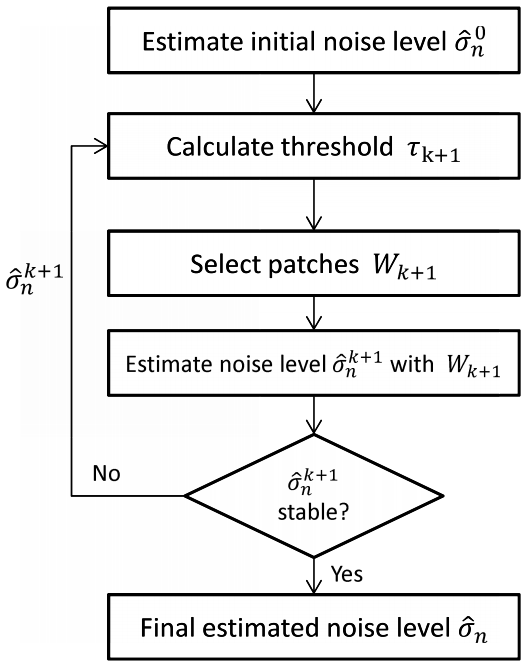
\includegraphics[width=0.9\columnwidth]{single_image_noise_estimation.png}
	\caption{Algorithm for \cite{noise-weak-texture}.}
	\label{fig:alg-weak-texture}
\end{figure}
Noise Level Estimation Using Weak Textured Patches of a Single Noisy Image\cite{noise-weak-texture} uses low rank weak textured patches without high frequency components. Noise level is then estimated from selected patches using principal component analysis(PCA). Figure \ref{fig:alg-weak-texture} shows the overall algorithm for this method.

\subsection{Filtering Framework}
SD Filter\cite{ham2015} utilizes both static and dynamic guidance images to preserve structure of the high detailed image and local features.

Filter will be tested on TRICLOBS\cite{triclobs} database. The database includes several captures of different wavelengths. Six scenarios will be tested:
\begin{itemize}
	\item LWIR as static guidance to NIR
	\item LWIR as static guidance to Visible
	\item NIR as static guidance to LWIR
	\item NIR as static guidance to Visible
	\item Visible as static guidance to LWIR
	\item Visible as static guidance to NIR
\end{itemize}

Source code of the filter is available on the web via github\cite{github:sdfilter}. The code will be used on this project. If playing with parameters is not enough to get good results, the source code will be modified.

\section{Experiments}
\subsection{Sigma Estimation Methods}
As the first part of this project, the sigma estimation methods are tested on a synthetic noisy image. Random noise with different sigma levels are added to the original noise-free image and the methods are evaluated.

For testing 100 noisy images are generated to simulate a static scene for \ref{ss:online-var}. Method \ref{ss:weak-tex} is called with its default settings; patch size 7, no decimation, 0.99 confidence threshold, and 3 iterations. Noise levels for this experiment are; 2, 5, 10, 20.

\begin{table}[h!]
	\centering
	\begin{tabular}{cccc}
		\toprule
		Sigma Value & Method & Estimated Value & Error Rate\\
		\midrule
		\multirow{2}{*}{\(\sigma=2\)} & Method1 & 1.99 & 0.52 \% \\
		& Method2 & 1.93 & 3.61 \% \\
		\multirow{2}{*}{\(\sigma=5\)} & Method1 & 4.87 & 2.56 \% \\
		& Method2 & 4.75 & 5.04 \% \\
		\multirow{2}{*}{\(\sigma=10\)} & Method1 & 9.59 & 4.07 \% \\
		& Method2 & 9.39 & 6.10 \% \\
		\multirow{2}{*}{\(\sigma=20\)} & Method1 & 18.79 & 6.04 \% \\
		& Method2 & 18.41 & 7.97 \% \\
		\multirow{2}{*}{\(\sigma=30\)} & Method1 & 27.68 & 7.72 \% \\
		& Method2 & 27.18 & 9.41 \% \\
		\bottomrule
	\end{tabular}
	\caption{Sigma Estimation Test Results}
	\label{tab:sigma-est}
\end{table}

\autoref{tab:sigma-est} shows results for this experiment. The results look promising for both methods. The problem with this experiment is that they might not hold true for actual sensor noise.


\subsection{Filter Performance Evaluation}
In this section, filters performance will be evaluated. For the first part of the project, filter is throughly evaluated to see if it will actually fit our goals or not.
{\small
\bibliographystyle{ieee}
\bibliography{egbib}
}

\end{document}
